\documentclass[xcolor=x11names,compress]{beamer}

\usepackage{graphicx}
\usepackage{epstopdf}
\usepackage{tikz}
\usepackage{caption}
\usepackage{subcaption}
\usepackage[polish]{babel}
\usepackage[utf8]{inputenc}
\usepackage[T1]{fontenc}
\usetikzlibrary{decorations.fractals}

%% Beamer Layout %%%%%%%%%%%%%%%%%%%%%%%%%%%%%%%%%%
%%  This Beamer template was created by Cameron Bracken.
%%  Anyone can freely use or modify it for any purpose
%%  without attribution.
%%
%%  Last Modified: January 9, 2009
\useoutertheme[subsection=false,shadow]{miniframes}
\useinnertheme{default}
\usefonttheme{serif}
\usepackage{palatino}

\setbeamerfont{title like}{shape=\scshape}
\setbeamerfont{frametitle}{shape=\scshape}

\setbeamercolor*{lower separation line head}{bg=DeepSkyBlue4} 
\setbeamercolor*{normal text}{fg=black,bg=white} 
\setbeamercolor*{alerted text}{fg=red} 
\setbeamercolor*{example text}{fg=black} 
\setbeamercolor*{structure}{fg=black} 
 
\setbeamercolor*{palette tertiary}{fg=black,bg=black!10} 
\setbeamercolor*{palette quaternary}{fg=black,bg=black!10} 

\renewcommand{\(}{\begin{columns}}
\renewcommand{\)}{\end{columns}}
\newcommand{\<}[1]{\begin{column}{#1}}
\renewcommand{\>}{\end{column}}
%%%%%%%%%%%%%%%%%%%%%%%%%%%%%%%%%%%%%%%%%%%%%%%%%%

\begin{document}

\section{\scshape Spis treści}
\begin{frame}
\title{Ewakuacja tunelu w warunkach pożaru}
%\subtitle{SUBTITLE}
\author{
	Jakub Rakoczy, Michał Rus\\
	{\it dr inż. Jarosław Wąs}\\
}
\date{
	\begin{tikzpicture}[decoration=Koch curve type 2] 
		\draw[DeepSkyBlue4] decorate{ decorate{ decorate{ (0,0) -- (3,0) }}}; 
	\end{tikzpicture}  
	\\
	\vspace{1cm}
	\today
}
\titlepage
\end{frame}

\begin{frame}[allowframebreaks]{Spis treści}
\tableofcontents
\end{frame}

\section{\scshape Analiza}

% ------------------

\subsection{Zagadnienie ewakuacji tunelu}
\begin{frame}{Zagadnienie ewakuacji tunelu}

\begin{enumerate}
  \item Znaczenie praktyczne.
  \item Szczególnie niebezpieczne warunki.
  \item Możliwość wirtualnej analizy zagrożeń.
\end{enumerate}

\end{frame}

% ------------------

\subsection{Studium problemu}
\begin{frame}{Studium problemu}

\begin{enumerate}
  \item Aspekt fizyczny:
  \begin{itemize}
    \item lokalizacja,
    \item warunki krytyczne.
  \end{itemize}
  \item Charakterystyki psychologiczne i fizjologiczne:
  \begin{itemize}
    \item reprezentacja anatomii,
    \item motoryka ewakuowanych,
    \item reakcja na zagrożenie.
  \end{itemize}
\end{enumerate}

\end{frame}
\section{\scshape Narzędzia}

\subsection{Użyte technologie i narzędzia}
\begin{frame}{Użyte technologie i narzędzia}
\end{frame}
\section{\scshape Model}

\subsection{Opis modelu}
\begin{frame}{Opis modelu}
\end{frame}

\subsection{Teoria proksemiki}
\begin{frame}{Teoria proksemiki}
\end{frame}

\subsection{Reprezentacja ewakuowanego}
\begin{frame}{Reprezentacja ewakuowanego}
\end{frame}

\subsection{Funkcja kosztu}
\begin{frame}{Funkcja kosztu}
\end{frame}
\section{\scshape Implementacja}

% ------------------------

\subsection{Wyzwania związane z implementacją logiki ewakuowanego}
\begin{frame}{Wyzwania związane z implementacją logiki ewakuowanego}
  \begin{enumerate}
    \item Dynamiczna reakcja na zagrożenie.
    \item Warunki krytyczne.
    \item Wybór wyjścia ewakuacyjnego.
  \end{enumerate}
\end{frame}

% ------------------------

\subsection{Dynamiczna reakcja na zmiany temperatury}
\begin{frame}{Dynamiczna reakcja na zmiany temperatury}
  \begin{figure}
    \centering
    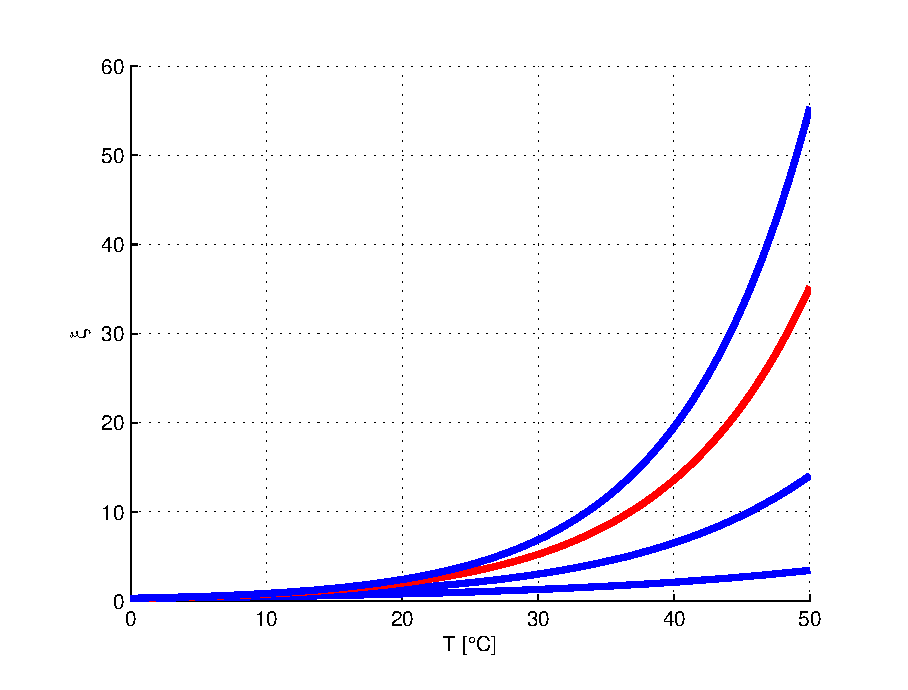
\includegraphics[height=0.6\textheight]{wykresy-kuba}
  \end{figure}
  $$\xi = \alpha \cdot B^T$$
  $\alpha = 0.3$, $B = 1.1$
\end{frame}

% ------------------------

\subsection{Warunki krytyczne --- stężenie CO}
\begin{frame}{Warunki krytyczne --- stężenie CO}
  \begin{figure}
    \centering
    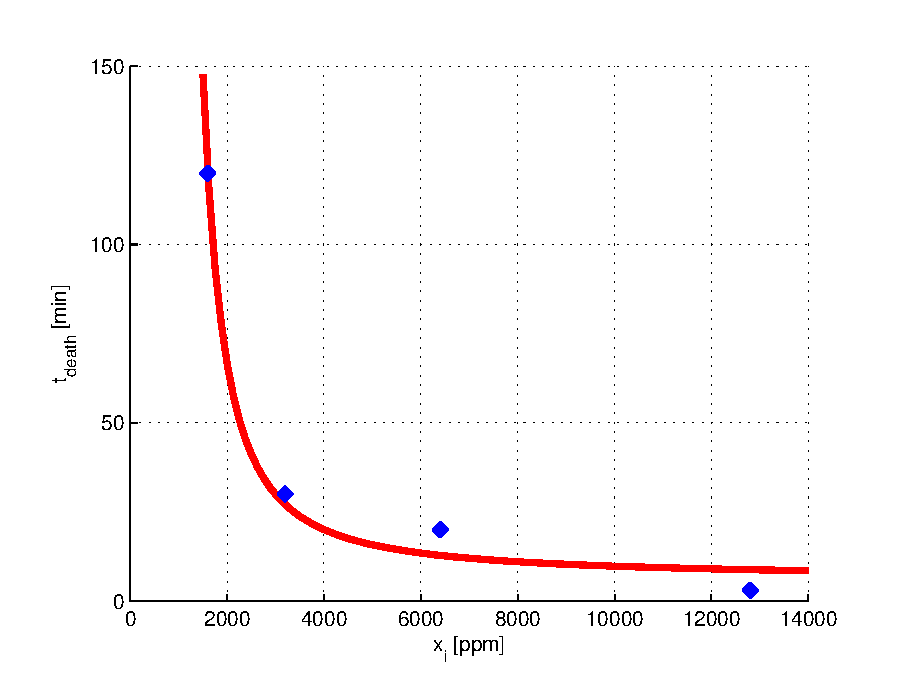
\includegraphics[height=0.6\textheight]{wykresy-wiki}
  \end{figure}
  $$HbCO_i = HbCO_{i-1} + HbCO_L \frac{CO_i}{CO_L}$$
  $HbCO_i$ -- aktualne stężenie karboksyhemoglobiny;
  $HbCO_{i-1}$ -- stężenie karboksyhemoglobinyw poprzedniej iteracji;
  $HbCO_L$ -- letalne stężenie karboksyhemoglobiny;
  $CO_i$ -- aktualne stężenieCO w powietrzu;
  $CO_L$ -- letalne stężenieCOw powietrzu.
\end{frame}
\section{\scshape Walidacja}

\subsection{Diagramy fundamentalne przepływów --- Hankin \&{} Wright, Weidmann}
\begin{frame}{Diagramy fundamentalne przepływów --- Hankin \&{} Wright, Weidmann}
  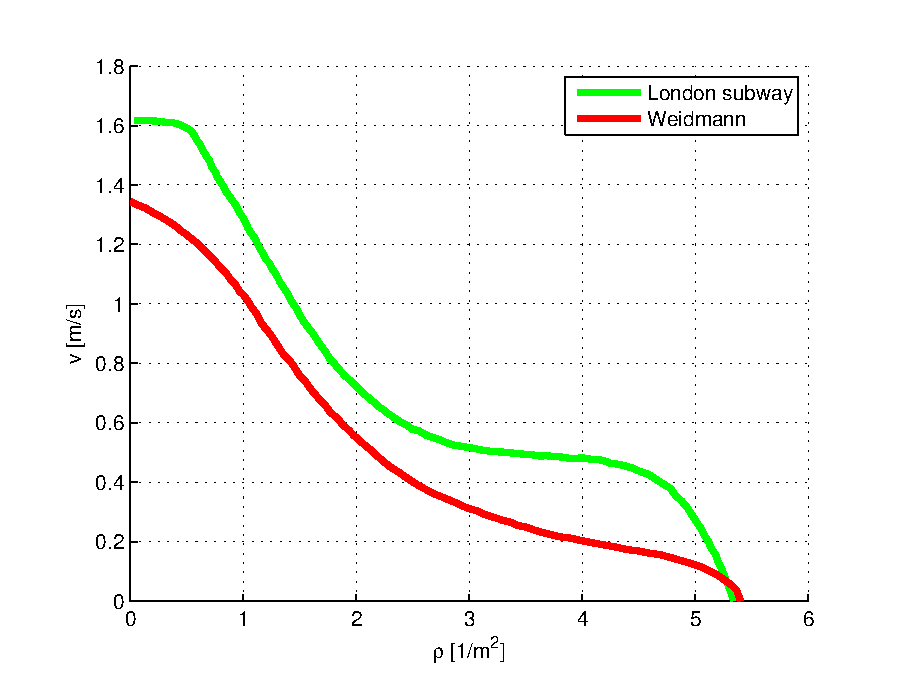
\includegraphics[width=\textwidth,height=0.8\textheight,keepaspectratio]{wykresy-hankin-wright}
\end{frame}

\subsection{Wąskie gardła --- Seyfried et al.}
\begin{frame}{Wąskie gardła --- Seyfried et al.}
  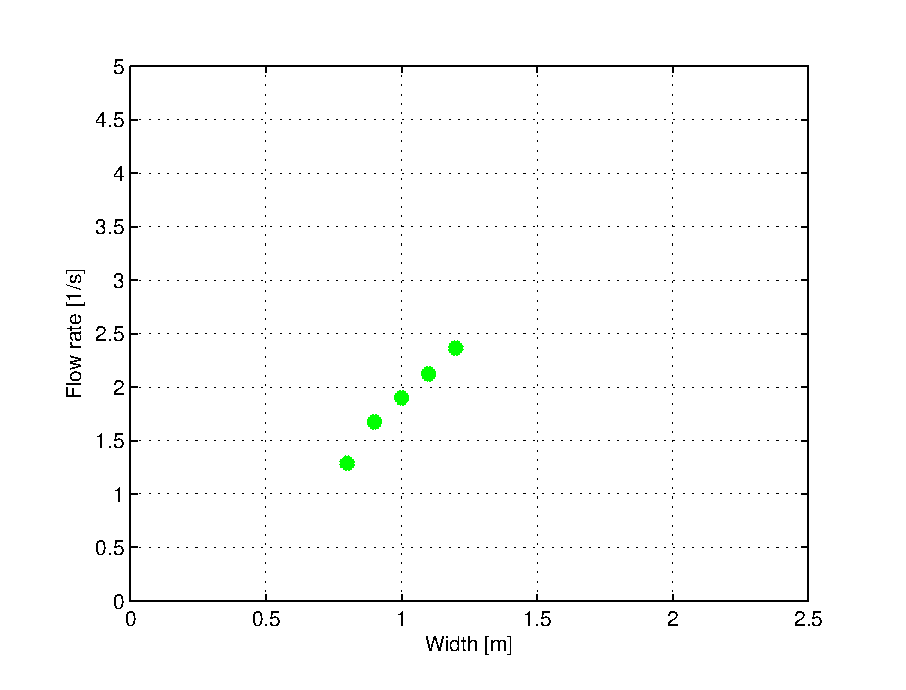
\includegraphics[width=\textwidth,height=0.8\textheight,keepaspectratio]{wykresy-seyfried}
\end{frame}

\subsection{Walidacja przepływu}
\begin{frame}{Walidacja przepływu}
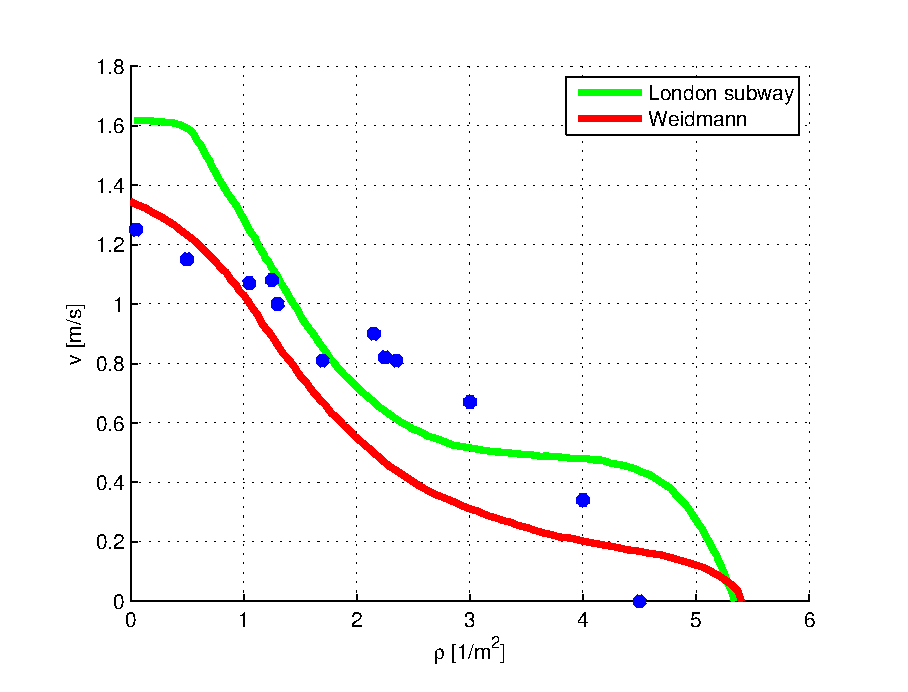
\includegraphics[width=\textwidth,height=0.8\textheight,keepaspectratio]{wykresy-weidmann_valid}
\end{frame}

\subsection{Bottleneck}
\begin{frame}{Bottleneck}

\begin{figure}
\centering
\begin{subfigure}{.5\textwidth}
  \centering
  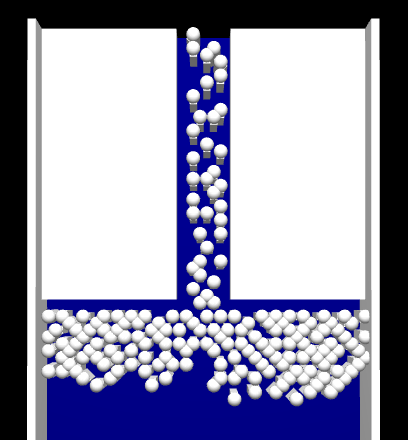
\includegraphics[width=.9\linewidth]{obrazek-bottleneck}
\end{subfigure}%
\begin{subfigure}{.5\textwidth}
  \centering
  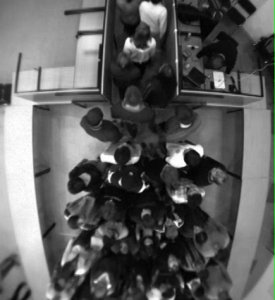
\includegraphics[width=.9\linewidth]{obrazek-bottleneck-real}
\end{subfigure}
\label{fig:test}
\end{figure}

\end{frame}

\subsection{Bottleneck validated}
\begin{frame}{Bottleneck validated}
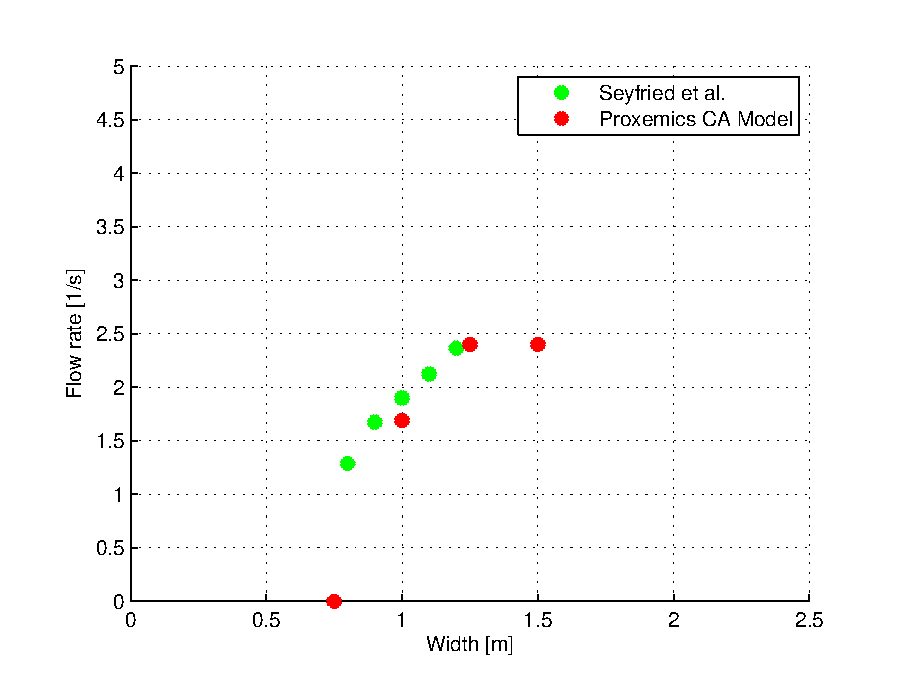
\includegraphics[width=\textwidth,height=0.8\textheight,keepaspectratio]{wykresy-bottleneck_validated}
\end{frame}
\section{\scshape Wnioski}

\subsection{Slajd 1}
\begin{frame}{Slajd 1}
\end{frame}

\subsection{Slajd 2}
\begin{frame}{Slajd 2}
\end{frame}
\section{\scshape Perspektywy}

\subsection{Perspektywy --- framework}
\begin{frame}{Perspektywy --- framework}
  \begin{itemize}
    \item Modularność.
    \item Dodanie modeli ciągłych.
    % TODO: screen?
    \item Porównanie modeli symulacyjnych pod względem wydajności i wyników.
    \item Automatyzacja procesów walidacji.
  \end{itemize}
\end{frame}

\section{\scshape Wykresy}

\subsection{Hankin-Wright}
\begin{frame}{Hankin-Wright}
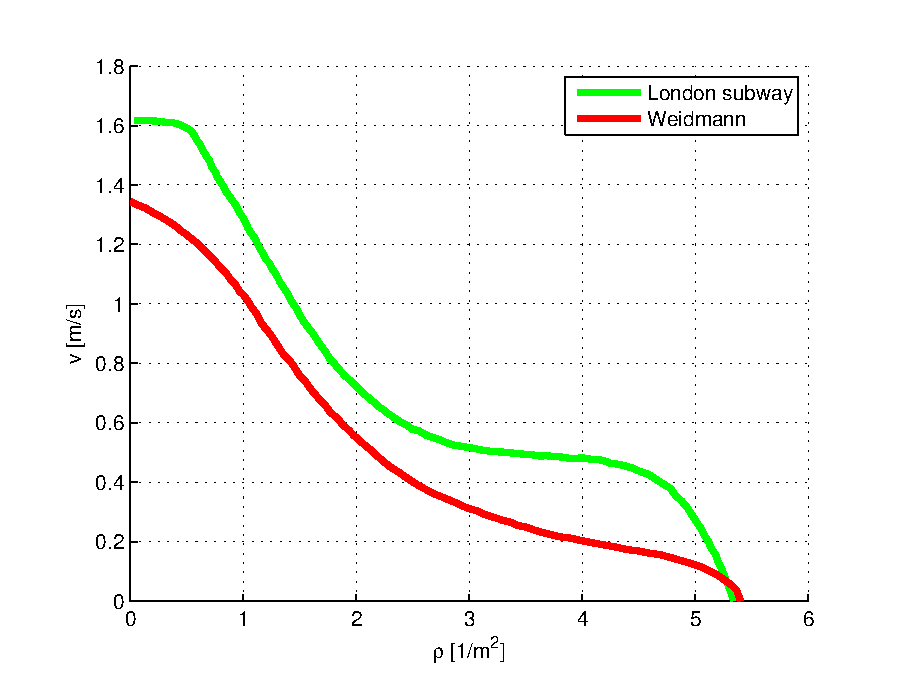
\includegraphics[width=\textwidth,height=0.8\textheight,keepaspectratio]{wykresy-hankin-wright}
\end{frame}

\subsection{Seyfried}
\begin{frame}{Seyfried}
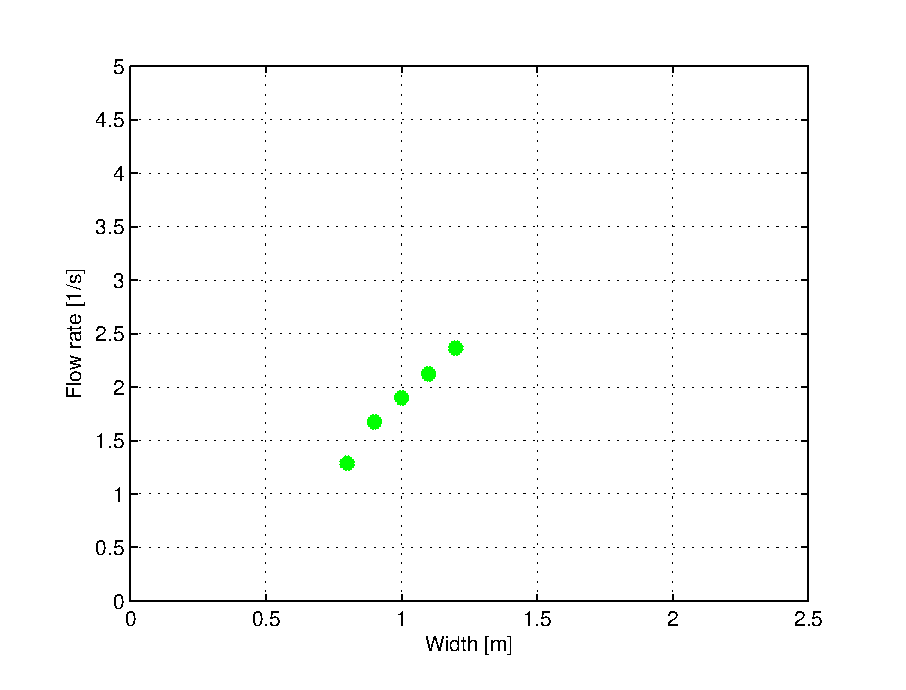
\includegraphics[width=\textwidth,height=0.8\textheight,keepaspectratio]{wykresy-seyfried}
\end{frame}

\subsection{Kuba}
\begin{frame}{Kuba}
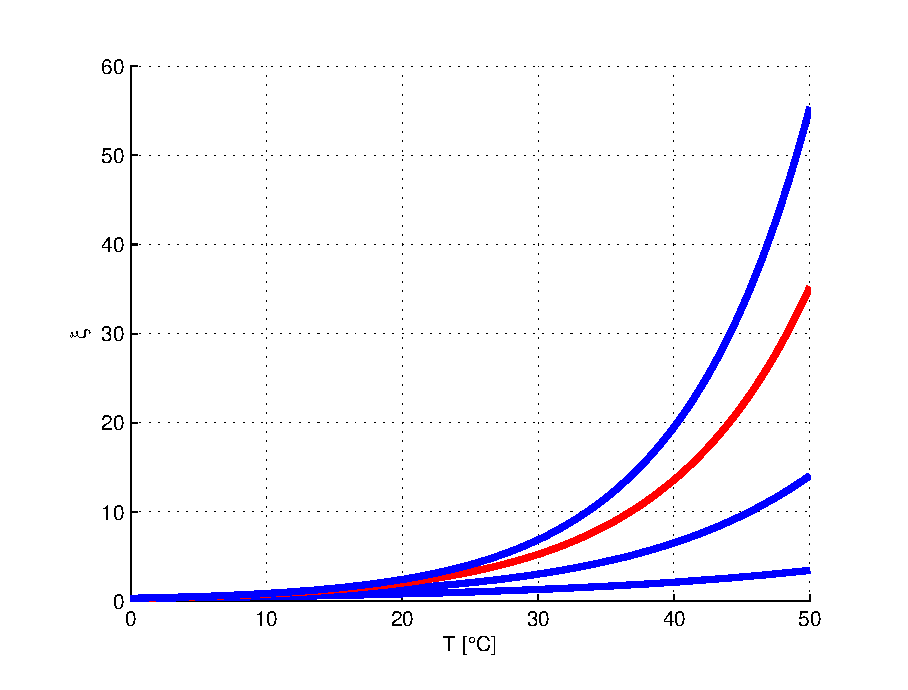
\includegraphics[width=\textwidth,height=0.8\textheight,keepaspectratio]{wykresy-kuba}
\end{frame}

\subsection{Wiki}
\begin{frame}{Wiki}
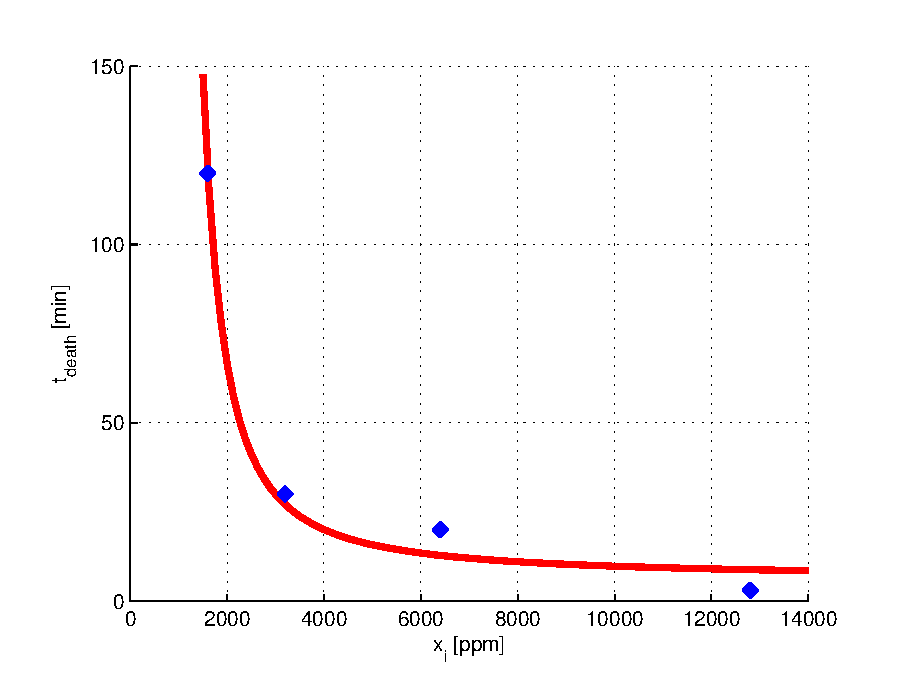
\includegraphics[width=\textwidth,height=0.8\textheight,keepaspectratio]{wykresy-wiki}
\end{frame}

\subsection{Walidacja przepływu}
\begin{frame}{Walidacja przepływu}
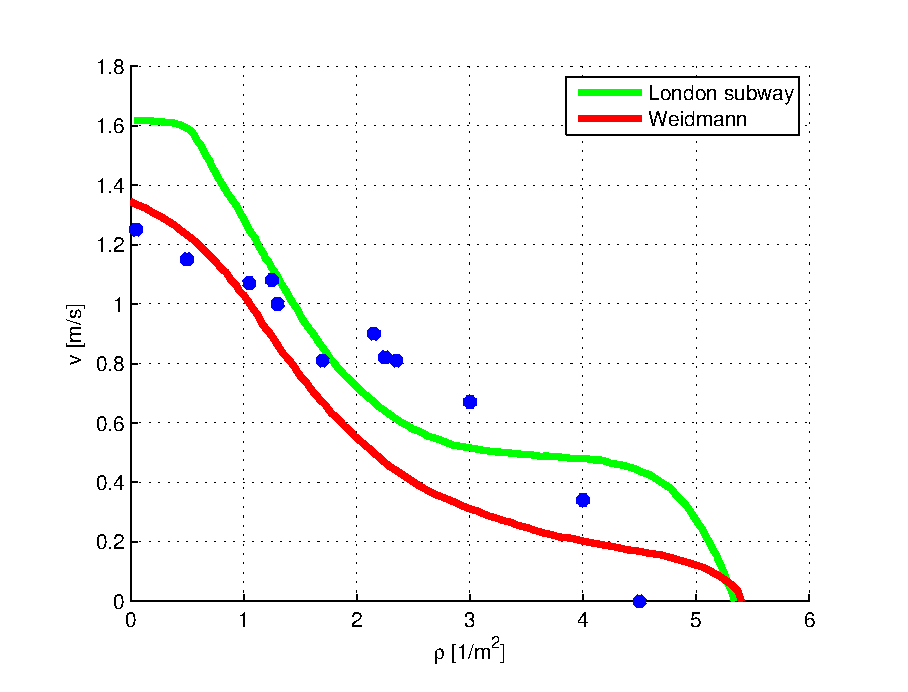
\includegraphics[width=\textwidth,height=0.8\textheight,keepaspectratio]{wykresy-weidmann_valid}
\end{frame}

\subsection{Bottleneck}
\begin{frame}{Bottleneck}

\begin{figure}
\centering
\begin{subfigure}{.5\textwidth}
  \centering
  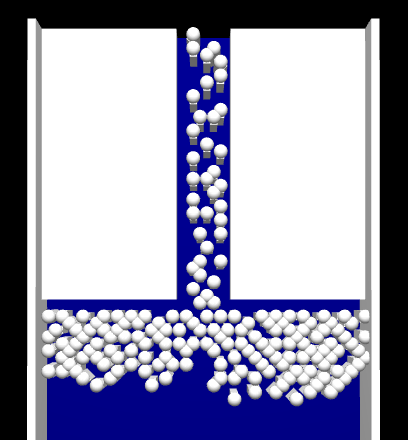
\includegraphics[width=.9\linewidth]{obrazek-bottleneck}
\end{subfigure}%
\begin{subfigure}{.5\textwidth}
  \centering
  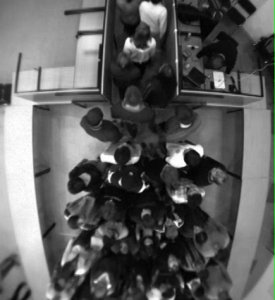
\includegraphics[width=.9\linewidth]{obrazek-bottleneck-real}
\end{subfigure}
\label{fig:test}
\end{figure}

\end{frame}

\end{document}